\documentclass[11pt]{article}

\usepackage[margin=1in]{geometry}
\usepackage{amsmath,amssymb,amsthm}
\usepackage{graphicx}
\usepackage[hidelinks]{hyperref}

\newtheorem{theorem}{Theorem}
\newtheorem{lemma}{Lemma}
\newtheorem{corollary}{Corollary}

\newcommand{\dist}{\operatorname{dist}}
\newcommand{\NA}{\operatorname{NA}}
\newcommand{\SE}{\operatorname{SE}}

\title{A Residual Set of Norm-Weak USC Points for \(M\)-Embedded Spaces}
\author{fa\_banach\_001, agent\_lane\_17}
\date{2026-06-20}

\begin{document}
\maketitle

\section*{Source Question}

In \emph{Computing sub differential limits of operators on Banach spaces},
arXiv:2212.09650, Rao studies norm-weak upper semicontinuity of the
preduality map. After recalling the state-space criterion of
Godefroy--Indumathi and proving results for \(M\)-ideals, the paper asks:

\begin{quote}
We do not know how to determine the largeness of points of norm-weak usc for
the preduality map on \(X^{**}\) in the category sense, when \(X\) is a
\(M\)-ideal in its bidual.
\end{quote}

\section*{Result}

The category answer is positive for every non-reflexive \(M\)-embedded Banach
space.

\begin{theorem}
Let \(X\) be a non-reflexive Banach space which is an \(M\)-ideal in its
bidual \(X^{**}\). Then the set of points of norm-weak upper semicontinuity for
the preduality map on \(X^{**}\) contains a dense \(G_\delta\) subset of
\(X^{**}\). In particular, the norm-weak usc points form a residual subset of
\(X^{**}\).
\end{theorem}

\section*{Idea of the Proof}

Rao's Proposition 9(b) already proves norm-weak usc at every
\(\tau\in X^{**}\) satisfying two conditions:

\[
  \tau \text{ attains its norm on } X^*
  \quad\text{and}\quad
  \dist(\tau,X)<\|\tau\|.
\]

The missing category observation is that, for \(M\)-embedded \(X\), these two
conditions hold simultaneously on a residual set. Indeed \(X^*\) has the
Radon--Nikodym property, so Bourgain's theorem, or equivalently the Stegall
variational principle in its standard norm-attainment form, gives a residual
set of norm-attaining functionals in \((X^*)^*=X^{**}\). The strict inequality
\(\dist(\tau,X)<\|\tau\|\) defines a dense open subset of \(X^{**}\). Their
intersection is dense \(G_\delta\), and Rao's proposition applies pointwise on
that intersection.

\section*{Proof}

\begin{proof}
We work over the real scalars, as in the source paper.

Let
\[
  \mathcal U=\{\tau\in X^{**}:\dist(\tau,X)<\|\tau\|\}.
\]
The set \(\mathcal U\) is open, because both \(\tau\mapsto \dist(\tau,X)\) and
\(\tau\mapsto \|\tau\|\) are norm-continuous.

\begin{lemma}
\(\mathcal U\) is dense in \(X^{**}\).
\end{lemma}

\begin{proof}
Fix \(\tau\in X^{**}\) and \(\varepsilon>0\). If
\(\dist(\tau,X)<\|\tau\|\), there is nothing to prove. Suppose instead that
\(\dist(\tau,X)=\|\tau\|=M\).

If \(M=0\), choose any nonzero \(x\in X\) with \(\|x\|<\varepsilon\). Then
\(\tau+x=x\in\mathcal U\).

Assume \(M>0\). Pick \(0<r<\varepsilon\). Choose \(x^*\in S_{X^*}\) such that
\(|\tau(x^*)|>M-r/3\). Then choose \(y\in S_X\) with
\(|x^*(y)|>2/3\), and replace \(y\) by \(-y\) if needed so that
\(\tau(x^*)+r x^*(y)\) has modulus greater than \(M\). Put \(x=ry\). Since
\(x\in X\), passage to the quotient by \(X\) gives
\[
  \dist(\tau+x,X)=\dist(\tau,X)=M.
\]
On the other hand,
\[
  \|\tau+x\|\ge |(\tau+x)(x^*)|>M.
\]
Thus \(\tau+x\in\mathcal U\) and \(\|\tau+x-\tau\|=r<\varepsilon\). Hence
\(\mathcal U\) is dense.
\end{proof}

Since \(X\) is \(M\)-embedded, \(X^*\) has the Radon--Nikodym property. By
Bourgain's theorem on RNP sets, in the form recalled by Jung--Martin--Rueda
Zoca, the absolutely strongly exposing scalar functionals on \(X^*\) form a
residual subset of \((X^*)^*=X^{**}\). Every such functional attains its norm
on \(X^*\). Therefore
\[
  \mathcal N=\{\tau\in X^{**}:\tau\text{ attains its norm on }X^*\}
\]
contains a dense \(G_\delta\) subset of \(X^{**}\).

Consequently \(\mathcal R=\mathcal U\cap\mathcal N\) contains a dense
\(G_\delta\) subset of \(X^{**}\). For every \(\tau\in\mathcal R\), Rao's
Proposition 9(b) applies directly: \(\tau\) attains its norm on \(X^*\) and
\(\dist(\tau,X)<\|\tau\|\), hence \(\tau\) is a point of norm-weak usc for the
preduality map on \(X^{**}\). Thus the norm-weak usc points contain a dense
\(G_\delta\) subset. Their complement is contained in the complement of this
dense \(G_\delta\), hence is meagre.
\end{proof}

\section*{Concrete Corollary}

Taking \(X=c_0(\Gamma)\), for any infinite set \(\Gamma\), gives
\(X^{**}=\ell_\infty(\Gamma)\). Thus the norm-weak usc points for the
preduality map on \(\ell_\infty(\Gamma)\) are residual. In this discrete
family there is also an explicit dense open subfamily: bounded functions whose
supremum norm is attained at one coordinate with a strict gap from all other
coordinates. The earlier \(c_0\)-only packet in this folder's history used this
concrete route; the theorem above subsumes it.

\section*{Verification and Limitations}

The proof uses three standard ingredients:

\begin{enumerate}
\item Rao's Proposition 9(b) from the source paper.
\item The standard structural fact that if \(X\) is \(M\)-embedded, then
      \(X^*\) has the Radon--Nikodym property.
\item Bourgain's RNP norm-attainment theorem, equivalently the Stegall
      variational principle in the form that absolutely strongly exposing
      scalar functionals on an RNP space form a residual subset of the dual.
\end{enumerate}

The theorem addresses the source paper's category question for non-reflexive
\(M\)-embedded Banach spaces. It does not address the separate operator-space
intermediate question in Remark 13 of the source paper.

\section*{Novelty Check}

Local index search for arXiv:2212.09650, norm-weak usc, preduality map, and
\(M\)-embedded category terms found only the earlier \(c_0\) partial packet
from this run. Web searches for exact phrases such as
\texttt{norm-weak usc preduality map M-embedded residual},
\texttt{preduality map M-ideal in its bidual category}, and
\texttt{norm-weak upper semi-continuity c0 preduality map} did not locate an
explicit statement of the full category answer. The proof is nevertheless a
short corollary of Rao's Proposition 9(b) and Bourgain--Stegall residual
norm-attainment.

\section*{Source Evidence}

\begin{center}
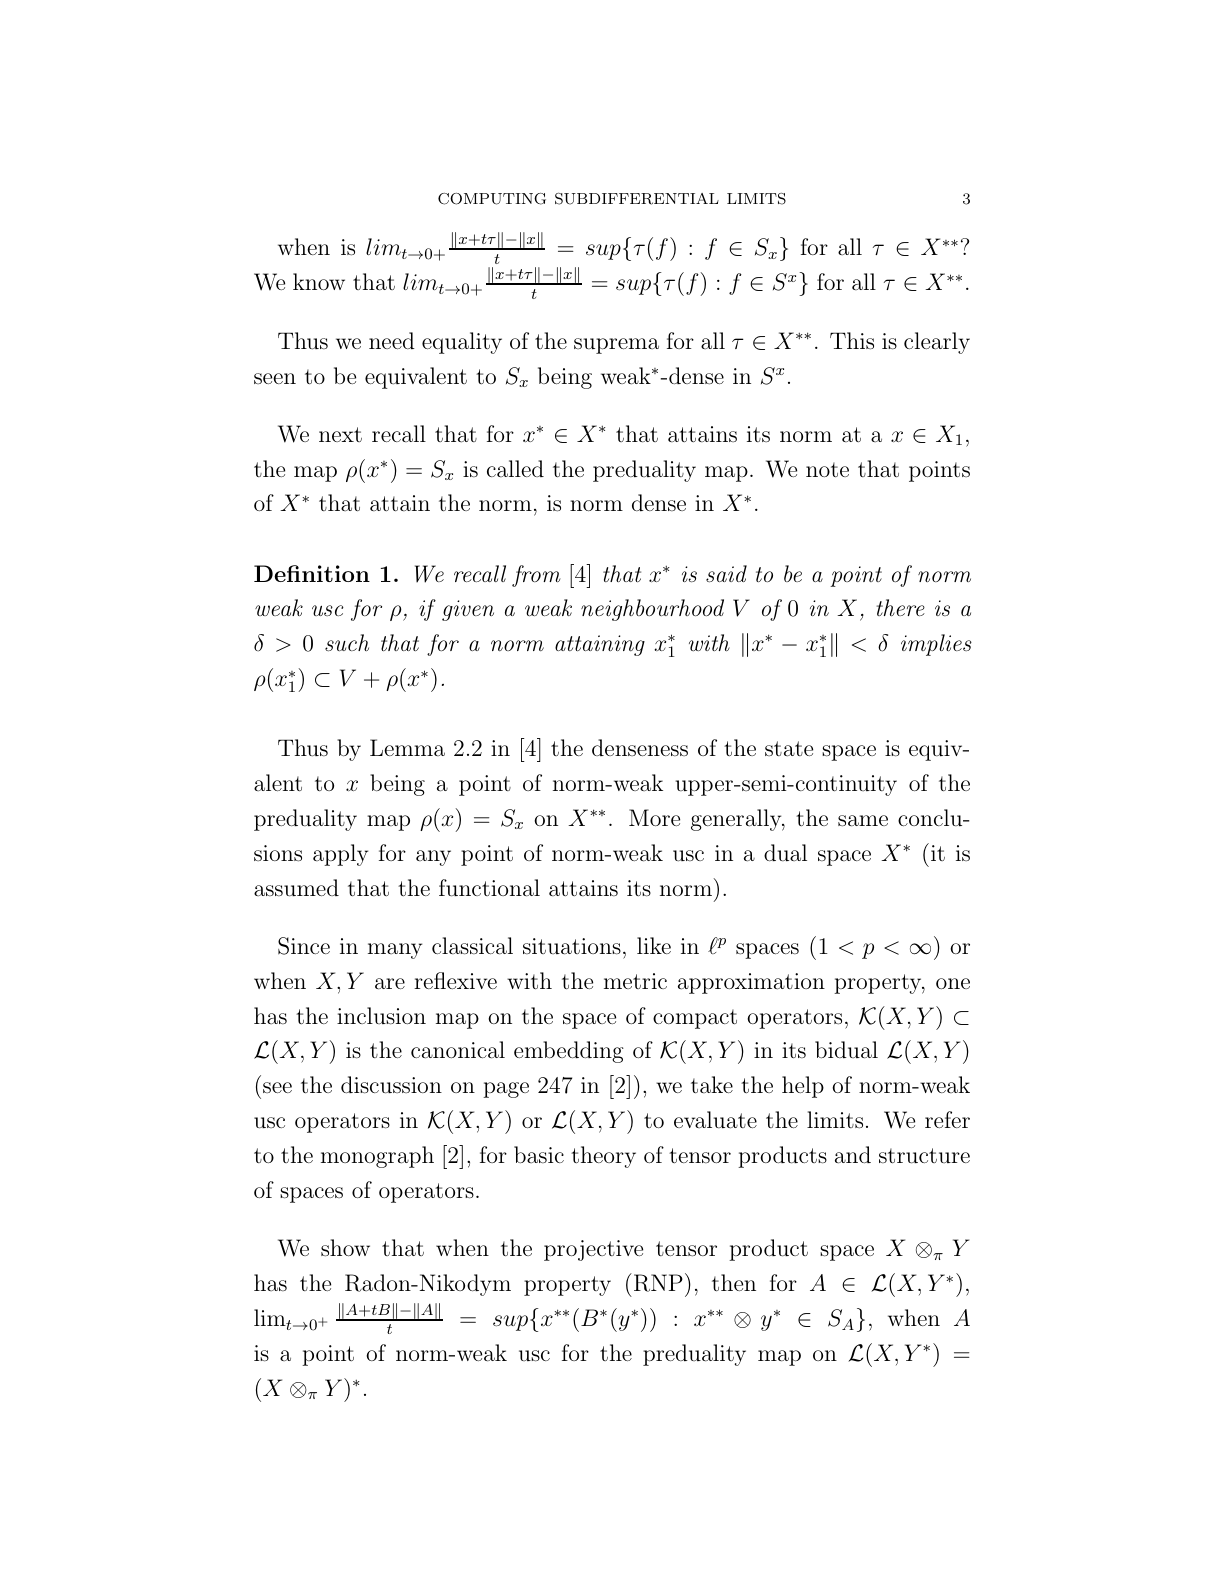
\includegraphics[width=.82\textwidth]{figures/definition_context_page3.png}
\end{center}

\begin{center}
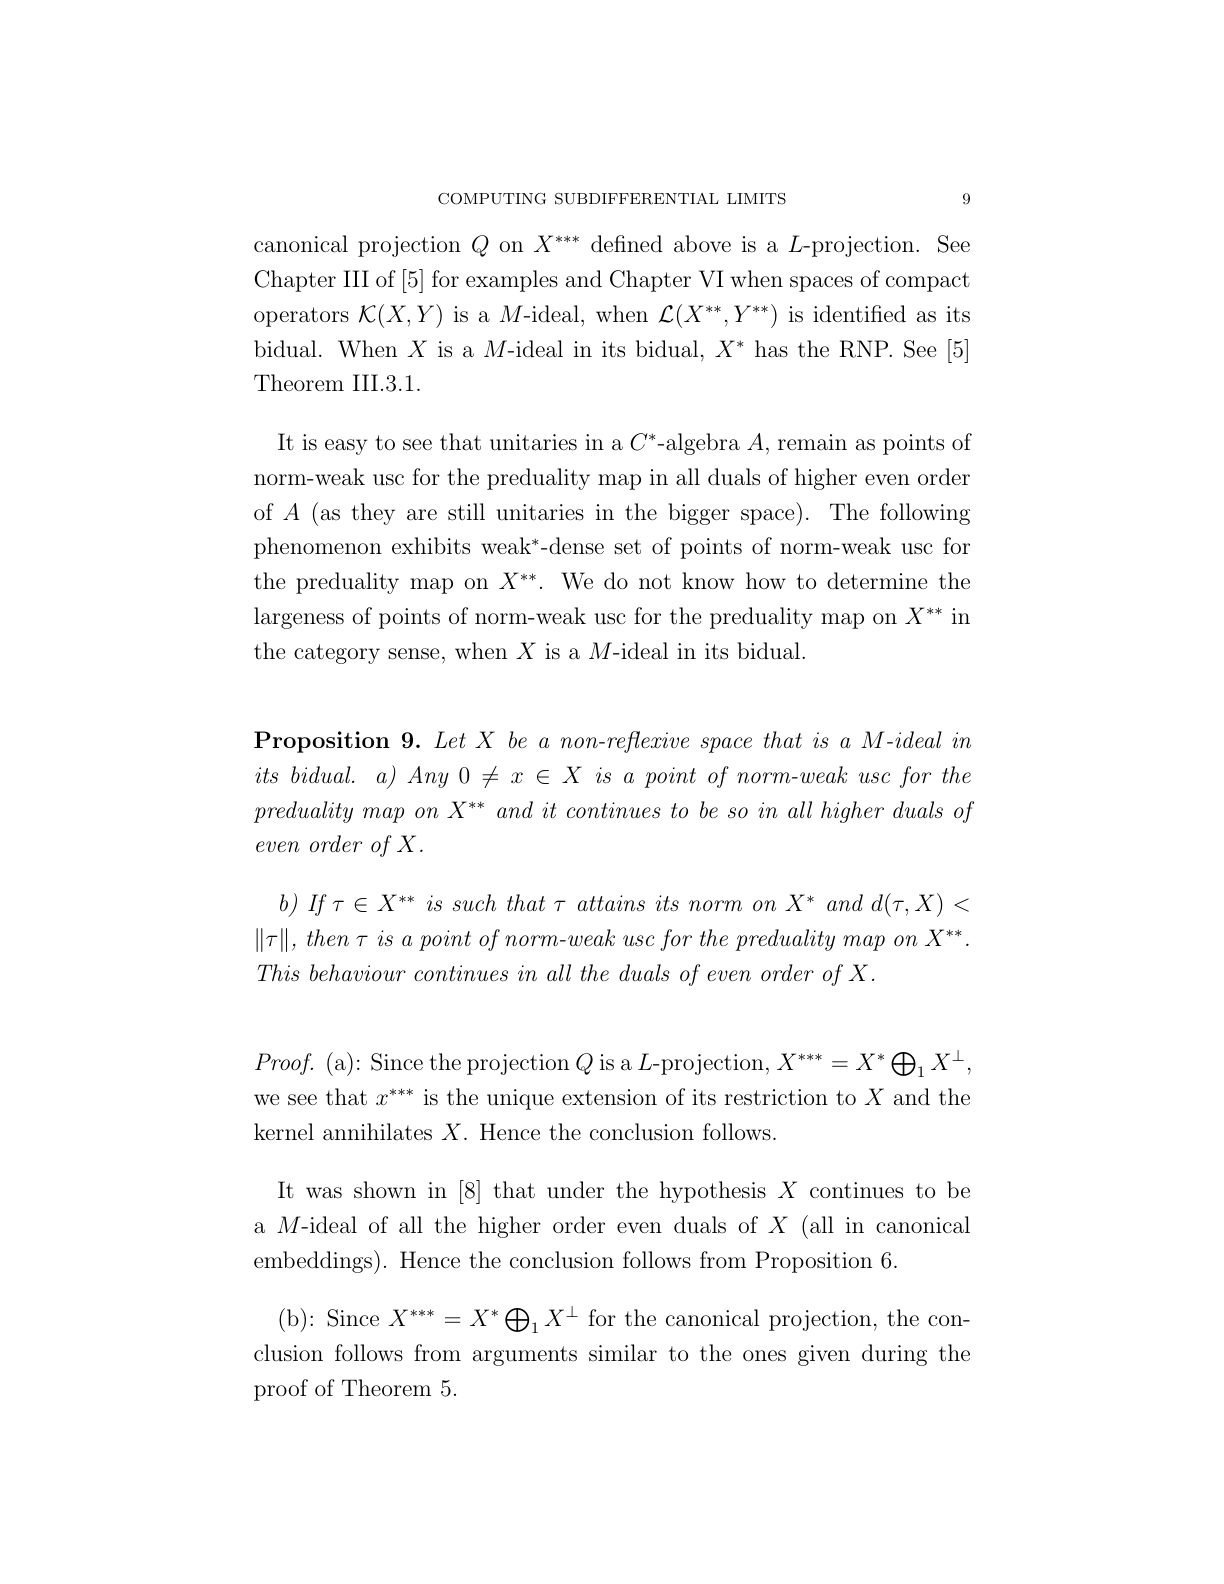
\includegraphics[width=.82\textwidth]{figures/open_problem_context_page9.png}
\end{center}

\section*{Human Review Recommendation}

Review as a claimed full solution to the category-largeness question after
Rao's Proposition 9. The main checks are:

\begin{enumerate}
\item confirm that the cited Bourgain--Stegall residual theorem applies to the
      Banach space \(X^*\);
\item confirm that the set \(\mathcal U=\{\tau:\dist(\tau,X)<\|\tau\|\}\) is
      dense in \(X^{**}\);
\item confirm that Rao's Proposition 9(b) has no additional hidden hypothesis
      beyond non-reflexive \(M\)-embeddedness, norm attainment on \(X^*\), and
      the strict distance inequality.
\end{enumerate}

\section*{References}

\begin{sloppypar}
\begin{enumerate}
\item T. S. S. R. K. Rao, \emph{Computing sub differential limits of operators
on Banach spaces}, arXiv:2212.09650, 2022.
\item G. Godefroy and V. Indumathi, \emph{Norm-to-weak upper semi-continuity of
the duality and pre-duality mappings}, Set-Valued Analysis 10 (2002), 317--330.
\item P. Harmand, D. Werner, and W. Werner, \emph{\(M\)-ideals in Banach spaces
and Banach algebras}, Lecture Notes in Mathematics 1547, Springer, 1993.
\item M. Jung, M. Martin, and A. Rueda Zoca, \emph{Residuality in the set of
norm attaining operators between Banach spaces}, J. Funct. Anal. 284 (2023),
Paper No. 109746; arXiv:2203.04023.
\end{enumerate}
\end{sloppypar}

\end{document}
